\documentclass[a4paper,12pt]{report}
\usepackage{graphicx}
\usepackage{amsmath}
\usepackage{booktabs}
\usepackage{float}
\usepackage{hyperref}
\usepackage{listings}
\usepackage{geometry}
\geometry{top=1in, bottom=1in, left=1in, right=1in}
\usepackage{fancyhdr}
\pagestyle{fancy}
\fancyhf{}
\fancyhead[L]{Báo cáo Tổng hợp cho LABs 1, 2, 3, và 4}
\fancyhead[R]{Tên sinh viên: Hoàng Lâm}

\title{Báo cáo Tổng hợp cho LABs 1, 2, 3, và 4}
\author{Sinh viên: Hoàng Lâm \\
Mã số sinh viên: QE180177 \\
Bộ môn: DAP391m \\
Giáo viên: Lê Võ Minh Thư \\
Ngày thực hiện: 21/10/2024}
\date{}

\begin{document}

\maketitle  % Generates the title page

\tableofcontents  % Generates the table of contents

\chapter{Giới thiệu}
Báo cáo này tổng hợp các kết quả và quá trình thực hiện của bốn Lab quan trọng trong hành trình nghiên cứu và phát triển hệ thống công nghệ. Các Lab này tập trung vào nhiều khía cạnh khác nhau, từ việc phát triển chatbot cơ bản, mở rộng các tính năng của chatbot, phân tích dữ liệu tiêu dùng sản phẩm công nghệ cho đến trực quan hóa dữ liệu không gian. Mỗi Lab không chỉ là một phần độc lập, mà còn kết nối chặt chẽ với nhau, giúp tạo ra một hệ sinh thái ứng dụng thông minh toàn diện hơn. 

Trong báo cáo này, chúng tôi sẽ lần lượt giới thiệu về từng Lab, những kỹ thuật đã áp dụng và phân tích giá trị của từng hệ thống.

\section{Lab 1: Phát triển hệ thống Chatbot cơ bản}
Lab 1 tập trung vào việc xây dựng hệ thống chatbot cơ bản, giúp người dùng có thể tương tác với một hệ thống tự động thông qua các câu hỏi đơn giản. Chúng tôi đã sử dụng các công nghệ như xử lý ngôn ngữ tự nhiên (Natural Language Processing - NLP) để hiểu và phản hồi các yêu cầu từ người dùng.

Chatbot cơ bản này mở ra cơ hội khám phá những gì mà công nghệ AI có thể làm được trong việc tương tác với con người. Nó cho phép làm quen với cơ sở hạ tầng của một hệ thống giao tiếp tự động, đồng thời xây dựng nền tảng cho các phiên bản chatbot phức tạp hơn sau này. Các tình huống hội thoại đơn giản trong Lab này tạo điều kiện cho việc tích hợp thêm các tính năng mở rộng.

\section{Lab 2: Mở rộng chức năng Chatbot với tư vấn sức khỏe và dinh dưỡng}
Sau khi xây dựng chatbot cơ bản, Lab 2 tập trung vào việc mở rộng hệ thống với các tính năng phức tạp hơn, cụ thể là khả năng cung cấp tư vấn sức khỏe và dinh dưỡng. Hệ thống không chỉ trả lời các câu hỏi đơn giản mà còn có khả năng lưu trữ thông tin người dùng, theo dõi và đưa ra lời khuyên chuyên sâu dựa trên lịch sử tương tác.

Việc mở rộng hệ thống chatbot với chức năng tư vấn sức khỏe đã đưa chatbot từ một hệ thống giao tiếp cơ bản trở thành một công cụ hỗ trợ hữu ích trong lĩnh vực chăm sóc sức khỏe. Phân tích và so sánh hiệu suất của các phương pháp lưu trữ và xử lý dữ liệu, giúp chatbot trở nên mượt mà và hiệu quả hơn.

\section{Lab 3: Phân tích và dự báo xu hướng tiêu dùng sản phẩm công nghệ}
Lab 3 là một bước tiến quan trọng trong việc khai thác dữ liệu. Quá trình phân tích bao gồm việc làm sạch dữ liệu, khám phá các mối tương quan giữa các biến số, và xây dựng các mô hình học máy (Machine Learning) để dự đoán xu hướng tiêu dùng trong tương lai. Chúng tôi đã sử dụng các mô hình như hồi quy tuyến tính (Linear Regression), cây quyết định (Decision Tree) và XGBoost để đánh giá chính xác xu hướng tiêu dùng.

Phân tích dữ liệu tiêu dùng công nghệ là một lĩnh vực quan trọng, giúp các doanh nghiệp dự đoán nhu cầu của thị trường và đưa ra các chiến lược kinh doanh hiệu quả. Việc ứng dụng các mô hình học máy trong Lab 3 giúp chúng tôi không chỉ hiểu được các xu hướng hiện tại mà còn dự đoán được xu hướng trong tương lai. Các mô hình như Hồi quy tuyến tính và XGBoost đã chứng minh được sự hiệu quả khi làm việc với các bộ dữ liệu lớn và phức tạp.

\section{Lab 4: Trực quan hóa dữ liệu không gian với Streamlit}
Lab 4 tập trung vào việc trực quan hóa dữ liệu không gian bằng cách phát triển ứng dụng web sử dụng Streamlit. Dữ liệu địa lý được thu thập từ các nguồn như OpenStreetMap và các bộ dữ liệu khác, sau đó được trình bày trên các bản đồ tương tác.

Việc trực quan hóa dữ liệu không gian giúp người dùng không chỉ nhìn thấy thông tin dưới dạng số liệu mà còn hiểu rõ hơn về mối quan hệ giữa các yếu tố địa lý và dữ liệu khác. Trong Lab này, chúng tôi đã tích hợp thêm các tính năng tương tác, cho phép người dùng tự do điều chỉnh các lớp bản đồ và xem các biến động theo thời gian thực. Ứng dụng Streamlit cung cấp một giao diện thân thiện và dễ sử dụng..

\chapter{Lab 1: Phát triển Hệ thống Chatbot Cơ bản}

\section{Giới thiệu}
Trong Lab 1, mục tiêu chính là phát triển một hệ thống chatbot cơ bản, tập trung vào việc hỗ trợ người dùng truy vấn thông tin về sức khỏe và dinh dưỡng. Chatbot này sử dụng nền tảng \textbf{Rasa} (Open souce platform) kết hợp với mô hình xử lý ngôn ngữ tự nhiên (NLP), cho phép cung cấp phản hồi theo ngữ cảnh và cải thiện trải nghiệm người dùng.

\section{Phân tích Hệ thống Chatbot}
Hệ thống được thiết kế để hỗ trợ các câu hỏi liên quan đến sức khỏe và dinh dưỡng, với khả năng ghi nhớ và duy trì ngữ cảnh của cuộc hội thoại trước đó. Một trong những ưu điểm của việc sử dụng Rasa là khả năng tùy chỉnh chatbot và tích hợp với các API và cơ sở dữ liệu khác nhau.

\section{Cấu trúc Hệ thống}
Chatbot được triển khai với các thành phần chính sau:
\begin{itemize}
    \item \textbf{Xử lý ngôn ngữ tự nhiên (NLP):} Rasa giúp phân tích và hiểu ngữ cảnh của câu hỏi để đưa ra câu trả lời phù hợp.
    \item \textbf{Kết nối cơ sở dữ liệu:} Dữ liệu người dùng và các câu hỏi được lưu trữ, giúp cá nhân hóa trải nghiệm của người dùng.
\end{itemize}

\section{Phân tích ưu/nhược điểm}

\textbf{Ưu điểm:}
\begin{itemize}
    \item Hệ thống dễ dàng mở rộng để xử lý nhiều loại câu hỏi khác nhau.
    \item Khả năng ghi nhớ ngữ cảnh giúp cải thiện sự tương tác với người dùng.
\end{itemize}

\textbf{Nhược điểm:}
\begin{itemize}
    \item Vẫn gặp khó khăn khi xử lý các câu hỏi phức tạp hoặc không đủ ngữ cảnh.
    \item Dữ liệu huấn luyện cần được mở rộng để chatbot hiểu sâu hơn các tình huống khác nhau.
\end{itemize}

\section{Kiểm thử và Đánh giá}
Quá trình kiểm thử tập trung vào khả năng phản hồi của chatbot đối với các câu hỏi về sức khỏe. Kết quả cho thấy chatbot có thể trả lời đúng các câu hỏi cơ bản, tuy nhiên hiệu suất giảm khi gặp các câu hỏi có tính phức tạp cao. Đề xuất cải tiến bao gồm:
\begin{itemize}
    \item \textbf{Tăng cường dữ liệu huấn luyện:} Cần bổ sung thêm nhiều ngữ cảnh và tình huống đa dạng để chatbot học hỏi.
    \item \textbf{Cải thiện khả năng giữ ngữ cảnh:} Điều chỉnh logic để chatbot có thể duy trì ngữ cảnh tốt hơn trong các cuộc hội thoại dài.
\end{itemize}

\begin{figure}[h]
    \centering
    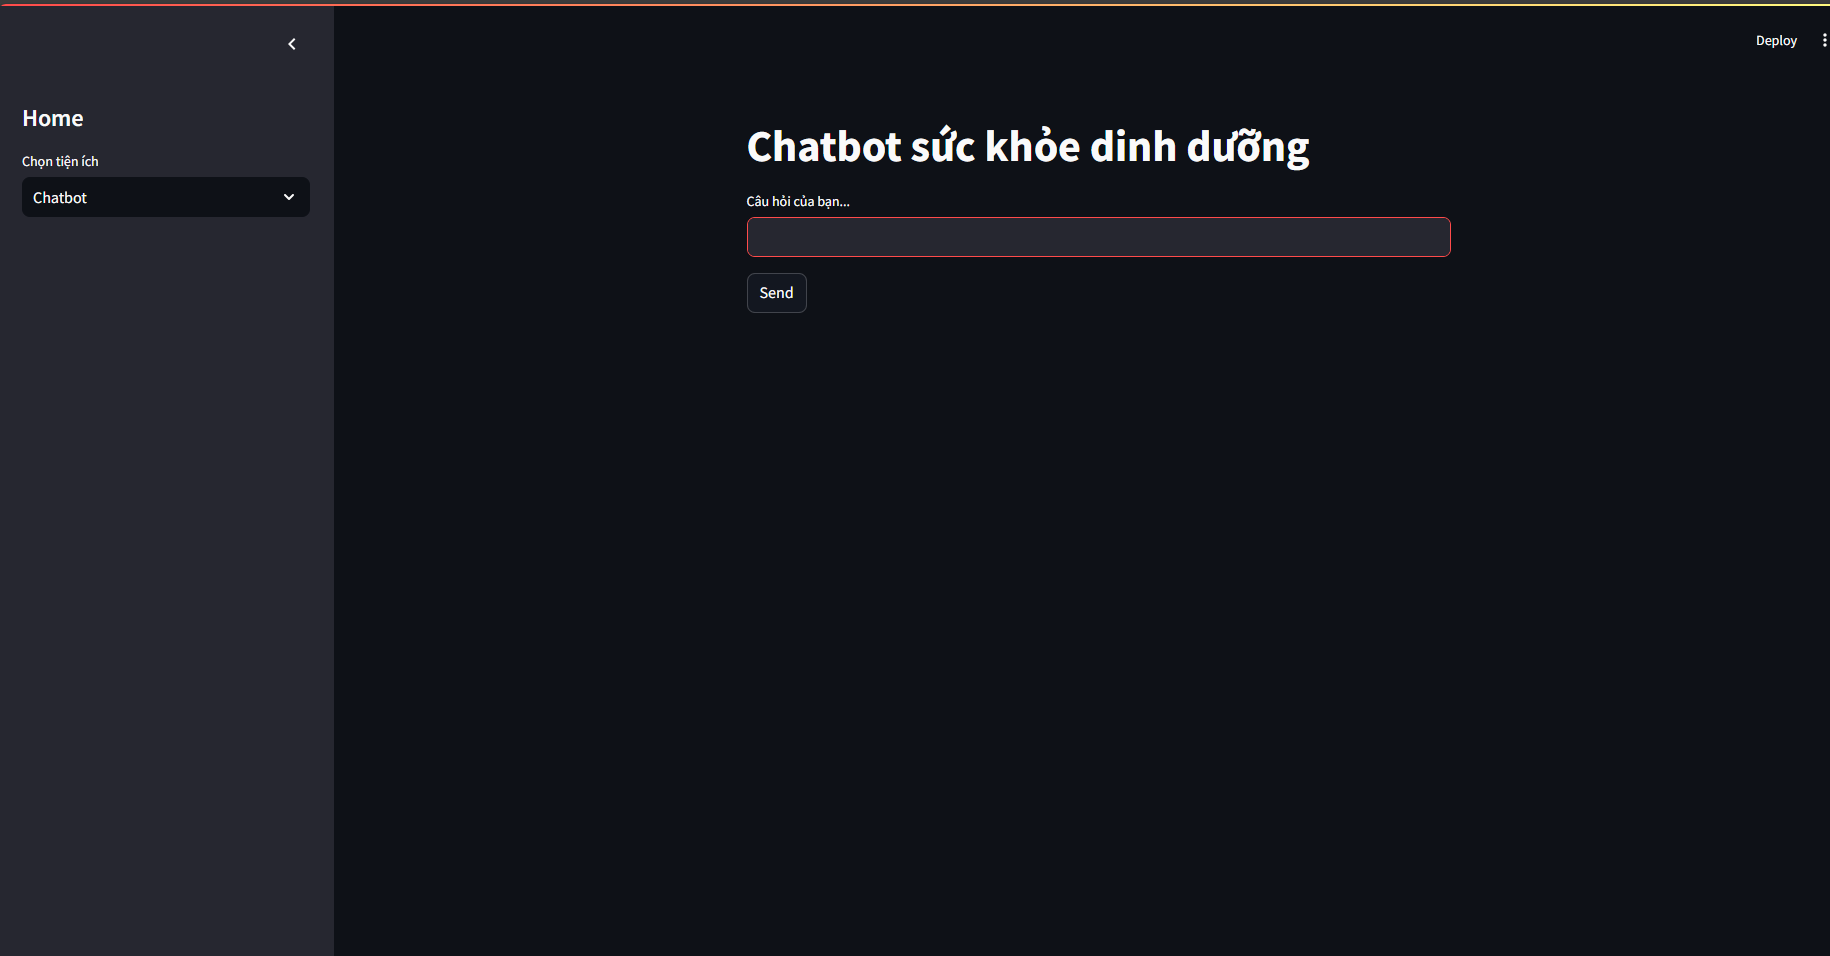
\includegraphics[width=0.5\textwidth]{image/home.png}
    \caption{Home}
    \label{fig:home}
\end{figure}


\section{Kết luận}
Lab 1 giúp chúng tôi hiểu rõ hơn về cách phát triển một hệ thống chatbot cơ bản và các thách thức liên quan. Việc tích hợp NLP và khả năng giữ ngữ cảnh là những điểm nổi bật của hệ thống, tuy nhiên, cần có thêm dữ liệu và cải thiện trong việc xử lý các ngữ cảnh phức tạp để tăng hiệu quả của chatbot.

Báo cáo Lab 1 không chỉ cung cấp các thông tin kỹ thuật về việc phát triển chatbot mà còn mang lại cái nhìn tổng quan về các bước kiểm thử và cải tiến hệ thống nhằm nâng cao hiệu quả và trải nghiệm người dùng.

\chapter{Lab 2: Phát triển hệ thống Chatbot tư vấn sức khỏe dinh dưỡng}
\section{Mở rộng chức năng Chatbot}
Trong LAB 2, chúng tôi đã tập trung phát triển hệ thống chatbot có khả năng tư vấn sức khỏe và dinh dưỡng. Các chức năng chính của hệ thống bao gồm:
\begin{itemize}
    \item Đăng nhập (Login) và đăng ký (Register).
    \item Màn hình chính (Home) để người dùng tương tác với chatbot.
    \item Kết nối cơ sở dữ liệu (Database) sử dụng MongoDB để lưu trữ thông tin người dùng và lịch sử tương tác.
    \item Quản lý tài khoản người dùng (Account Management) cho phép cập nhật thông tin cá nhân và thay đổi mật khẩu.
\end{itemize}

\section{Quy trình phát triển}
Trong quá trình phát triển hệ thống, chúng tôi đã sử dụng MongoDB để lưu trữ dữ liệu người dùng. Điều này giúp hệ thống mở rộng dễ dàng và hiệu quả khi có số lượng lớn người dùng. Các chức năng chính được triển khai bằng ngôn ngữ Python và các thư viện liên quan như Flask để tạo các API xử lý yêu cầu từ chatbot.

\subsection{Mã kiểm tra thông tin đăng nhập}
Dưới đây là đoạn mã nguồn kiểm tra thông tin đăng nhập từ cơ sở dữ liệu MongoDB:

\begin{verbatim}
from pymongo import MongoClient

def check_account_credentials(username, password):
    uri = "mongodb+srv://<your_mongo_uri>"
    client = MongoClient(uri)
    db = client['chatbot']
    collection = db['account']
    user_document = collection.find_one({"user": username})
    client.close()
    if user_document and user_document.get("pass") == password:
        return True
    return False
\end{verbatim}

Mã trên giúp hệ thống xác minh thông tin người dùng và xử lý yêu cầu đăng nhập dựa trên cơ sở dữ liệu.

\section{Phân tích giao diện người dùng}
Sau khi phát triển hệ thống, chúng tôi tiến hành đánh giá giao diện người dùng (UI/UX) để đảm bảo tính trực quan và dễ sử dụng. Một số điểm cần cải thiện bao gồm:
\begin{itemize}
    \item Tối ưu hóa màu sắc và thiết kế đơn giản để người dùng dễ thao tác.
    \item Tích hợp thông báo (notification) để hướng dẫn người dùng trong quá trình sử dụng chatbot.
\end{itemize}

\section{Kết quả và đánh giá}
Việc tích hợp các chức năng mới đã cải thiện đáng kể hiệu suất của chatbot, giúp người dùng dễ dàng truy vấn thông tin về sức khỏe và dinh dưỡng. Tuy nhiên, một số điểm vẫn có thể được cải thiện, đặc biệt là về tốc độ xử lý và trải nghiệm người dùng khi sử dụng trên thiết bị di động.

Dưới đây là kết quả:

\begin{figure}[h]
    \centering
    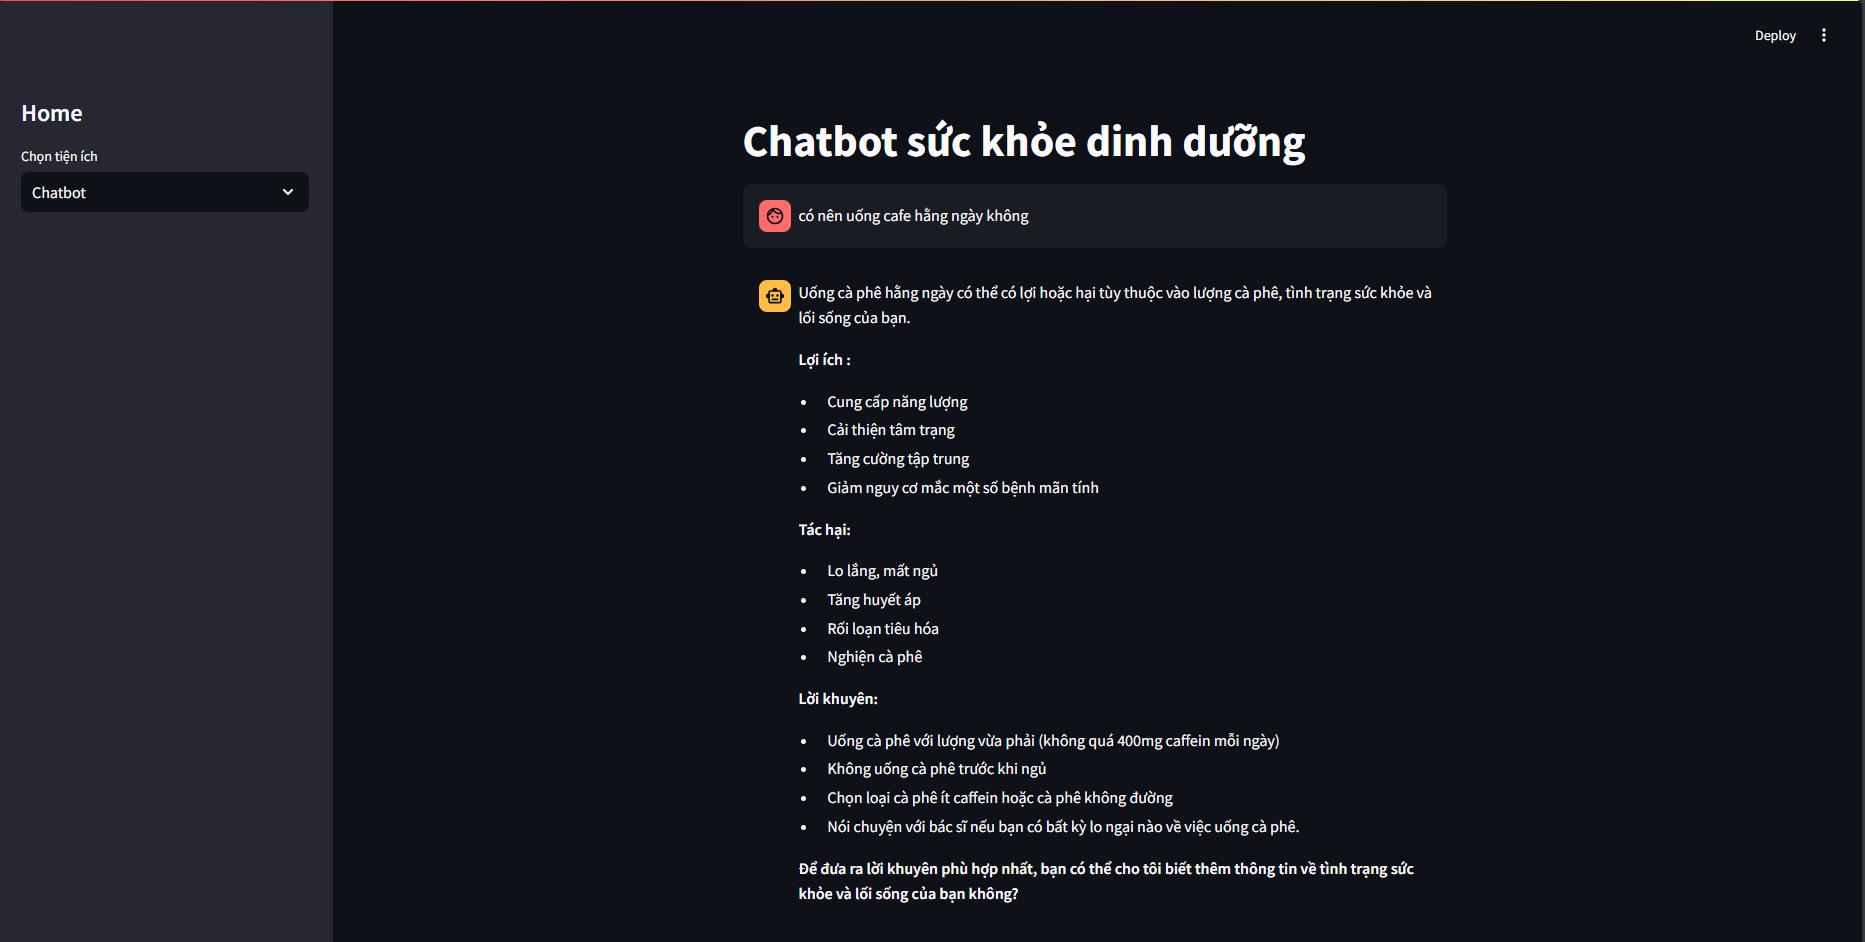
\includegraphics[width=0.5\textwidth]{image/home_lab01.png}
    \caption{Home}
    \label{fig:home_1}
\end{figure}

\begin{figure}[h]
    \centering
    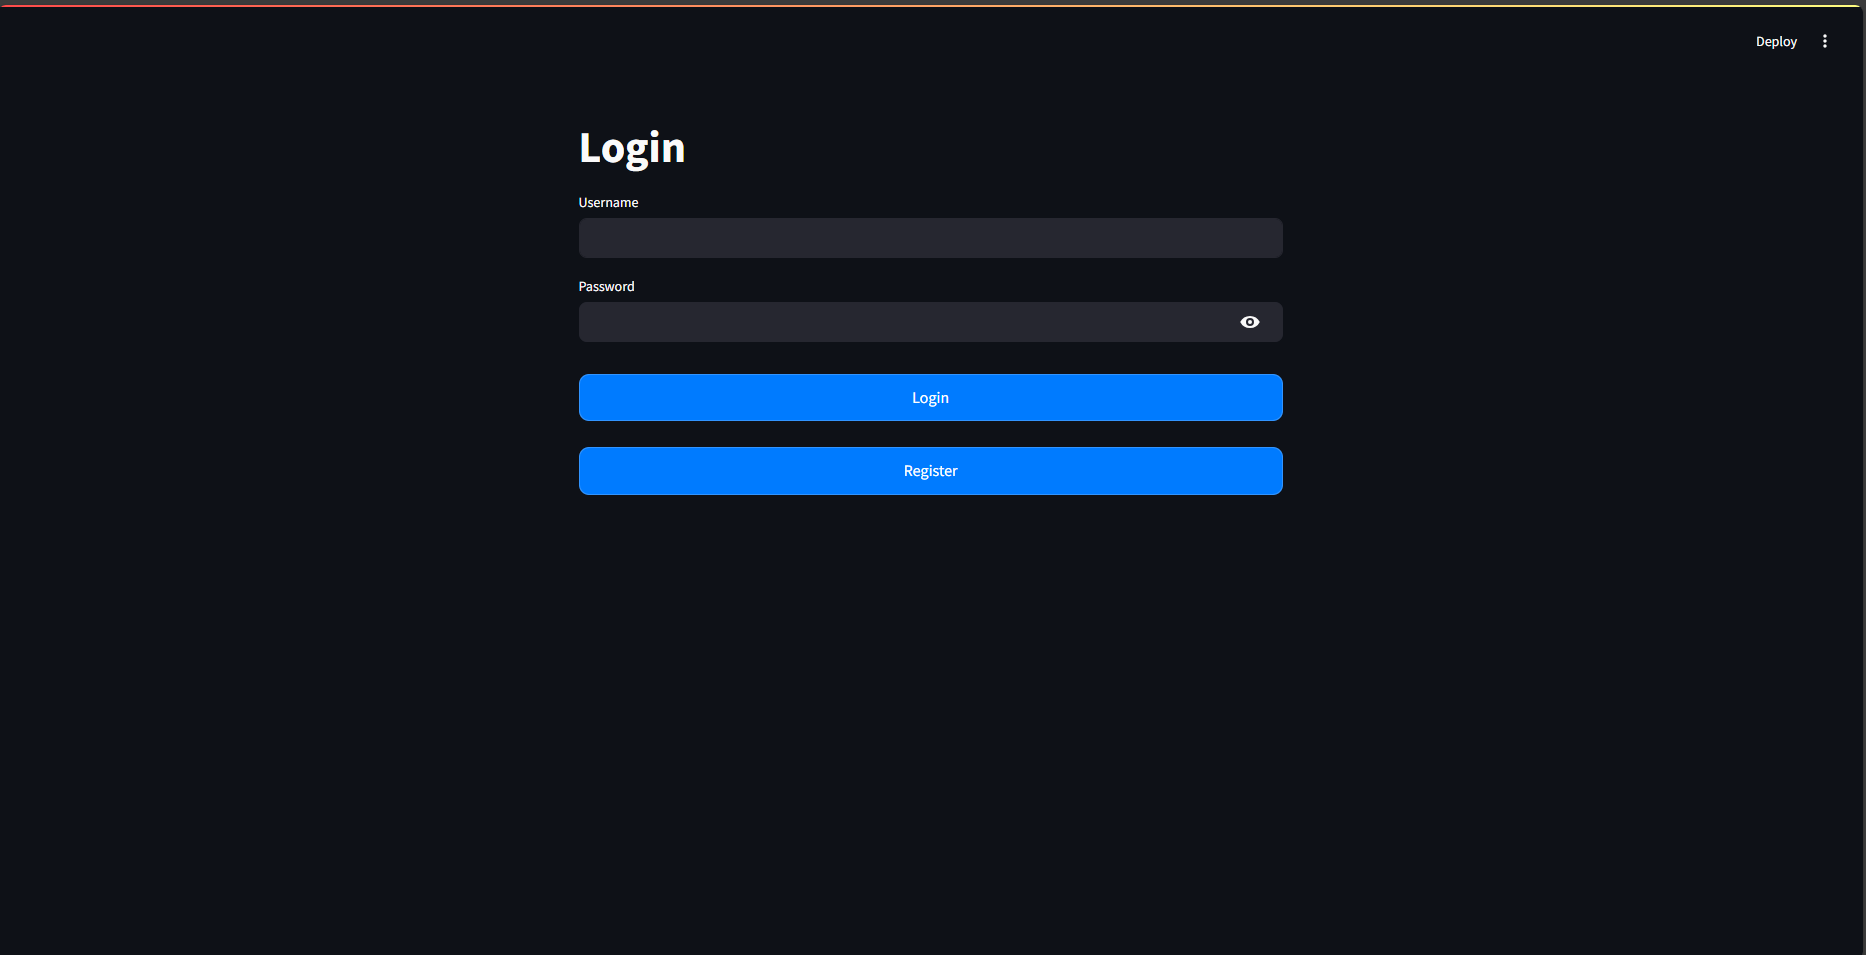
\includegraphics[width=0.5\textwidth]{image/login.png}
    \caption{Login}
    \label{fig:login}
\end{figure}

\begin{figure}[h]
    \centering
    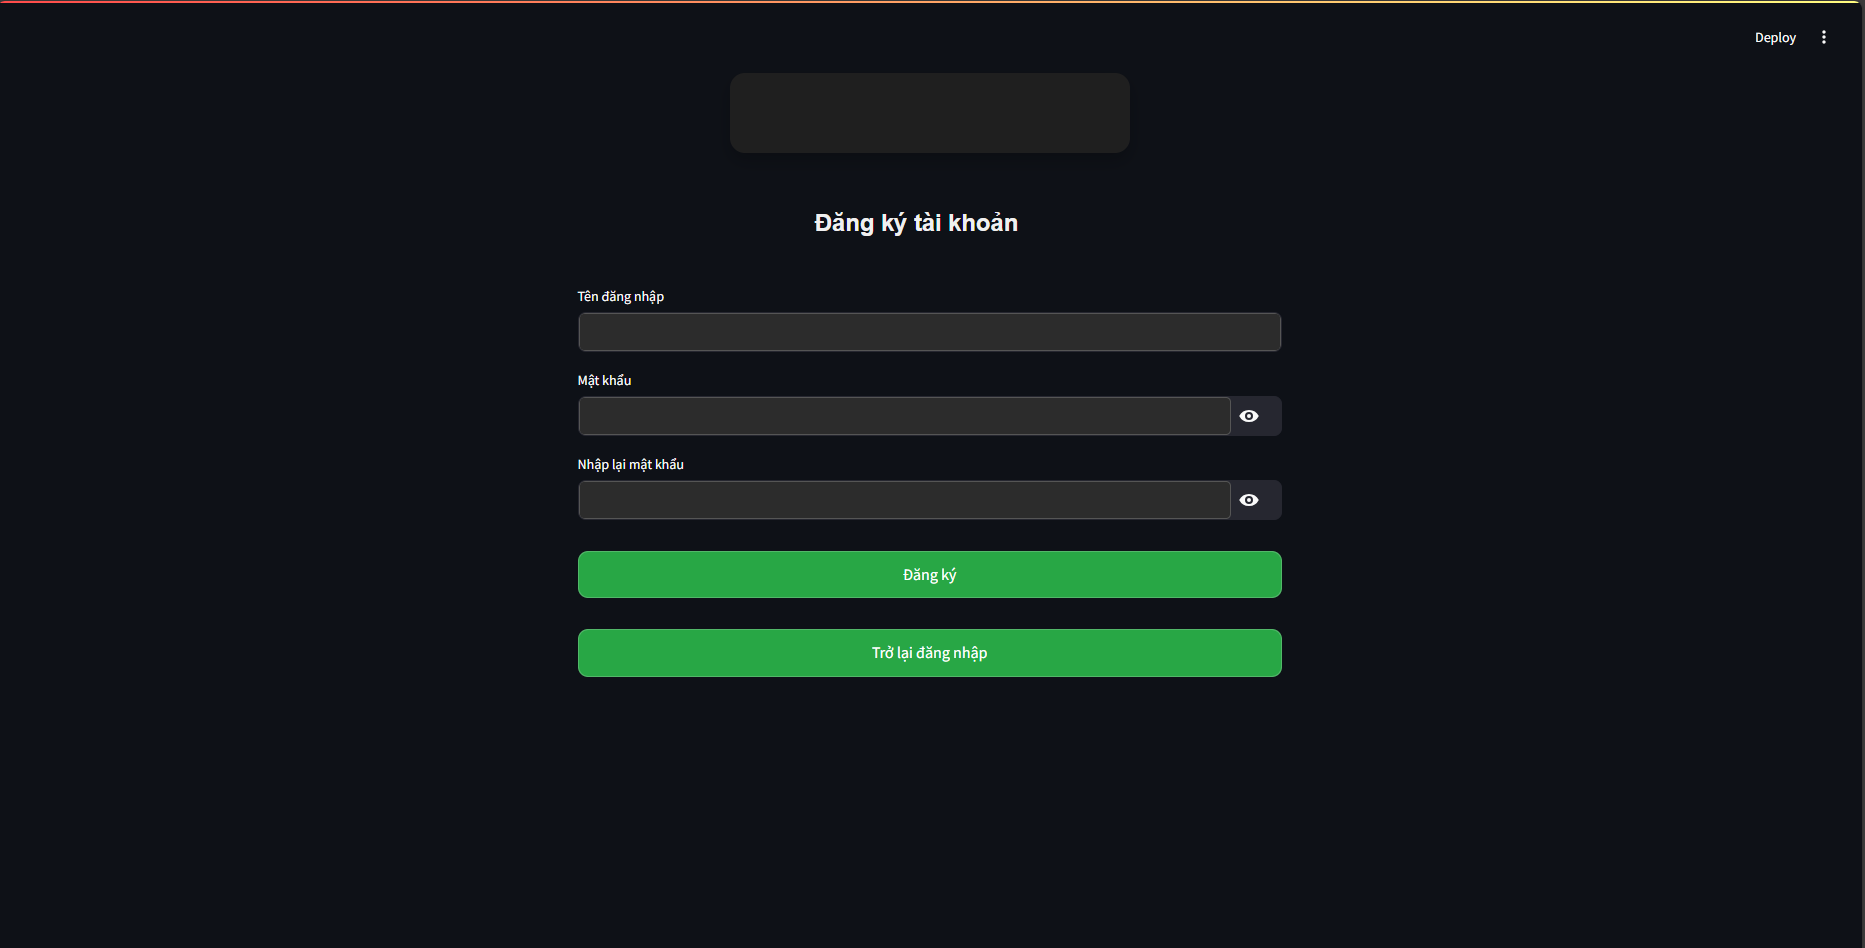
\includegraphics[width=0.5\textwidth]{image/register.png}
    \caption{Register}
    \label{fig:register}
\end{figure}

\section{Kết luận}
LAB 2 đã cho thấy tiềm năng trong việc ứng dụng chatbot vào các lĩnh vực như sức khỏe và dinh dưỡng. Việc mở rộng hệ thống chatbot không chỉ tăng cường khả năng tương tác với người dùng mà còn cung cấp các dịch vụ tư vấn cá nhân hóa. Chúng tôi nhận thấy rằng việc cải thiện giao diện và tối ưu hóa hiệu suất là các bước tiếp theo để hệ thống trở nên hoàn thiện hơn.

\chapter{Lab 3: Phân Tích và Dự Báo Xu Hướng Tiêu Dùng Sản Phẩm Công Nghệ}

\section{Giới thiệu}
Trong thời đại cách mạng công nghệ 4.0, xu hướng tiêu dùng các sản phẩm công nghệ liên tục thay đổi và phát triển. Việc phân tích các dữ liệu tiêu dùng giúp các doanh nghiệp trong ngành hiểu rõ hơn về nhu cầu của thị trường, từ đó tối ưu hóa các chiến lược kinh doanh. Báo cáo này tập trung vào việc thu thập, làm sạch và phân tích dữ liệu tiêu dùng sản phẩm công nghệ từ các nguồn uy tín, đồng thời sử dụng các mô hình học máy (Machine Learning) để dự báo xu hướng tiêu dùng trong tương lai.

Mục tiêu chính của báo cáo là:
\begin{itemize}
    \item Thu thập và làm sạch dữ liệu tiêu dùng từ nhiều nguồn khác nhau.
    \item Phân tích mối quan hệ giữa các biến số trong dữ liệu bằng các phương pháp khám phá dữ liệu (EDA).
    \item Sử dụng các mô hình học máy để dự đoán tình trạng sức khỏe của người dùng.

\end{itemize}

\section{Thu Thập và Làm Sạch Dữ Liệu}

\subsection{Thu Thập Dữ Liệu}
Tập dữ liệu chăm sóc sức khỏe tổng hợp của. Nó được thu thập dữ liệu chăm sóc sức khỏe trong thế giới thực, cho phép người dùng thực hành, phát triển và thể hiện kỹ năng phân tích và thao tác dữ liệu của họ trong bối cảnh ngành chăm sóc sức khỏe.(CSV, JSON, API, v.v.). Các biến số chính trong dữ liệu bao gồm:
\begin{itemize}
    \item Test result: Mô tả kết quả xét nghiệm y tế được thực hiện trong quá trình bệnh nhân nhập viện
    \item Age: Tuổi của bệnh nhân
    \item Blood: Nhóm máu
    \item Gender: Giới tính
    \item Medical Condition: Tình trạng bệnh lý chính hoặc chẩn đoán liên quan đến bệnh nhân
    \item Insurance Provider: Bảo hiểm của bệnh nhân
    \item Billing Amount: Số tiền được thanh toán cho các dịch vụ chăm sóc sức khỏe của bệnh nhân trong thời gian họ nhập viện
\end{itemize}

Dữ liệu được lưu trữ dưới dạng bảng với các hàng đại diện cho các điểm dữ liệu riêng lẻ. Sau khi thu thập, dữ liệu này cần được làm sạch và chuẩn hóa trước khi đưa vào phân tích.

\subsection{Làm Sạch Dữ Liệu}
Quá trình làm sạch dữ liệu là một bước quan trọng để đảm bảo tính chính xác của các phân tích và dự đoán. Các bước làm sạch dữ liệu bao gồm:
\begin{itemize}
    \item \textbf{Loại bỏ dữ liệu thiếu}: Những bản ghi không đầy đủ hoặc thiếu thông tin quan trọng sẽ được loại bỏ hoặc điền vào dựa trên các quy tắc tính toán.
    \item \textbf{Phát hiện và xử lý ngoại lệ (outliers)}: Các giá trị bất thường có thể làm sai lệch kết quả phân tích, do đó cần phát hiện và xử lý kịp thời.
    \item \textbf{Chuẩn hóa dữ liệu}: Để đảm bảo tính đồng nhất của các biến số, các giá trị như giá cả và mức tiêu thụ được chuẩn hóa về cùng một đơn vị.
\end{itemize}

\section{Phân Tích Khám Phá Dữ Liệu (EDA)}

\subsection{Phân Tích Mối Quan Hệ Giữa Các Biến}
Trong quá trình phân tích khám phá dữ liệu, chúng tôi đã sử dụng các biểu đồ cột để xác định mối quan hệ giữa các biến trong dữ liệu.

\begin{figure}[h]
    \centering
    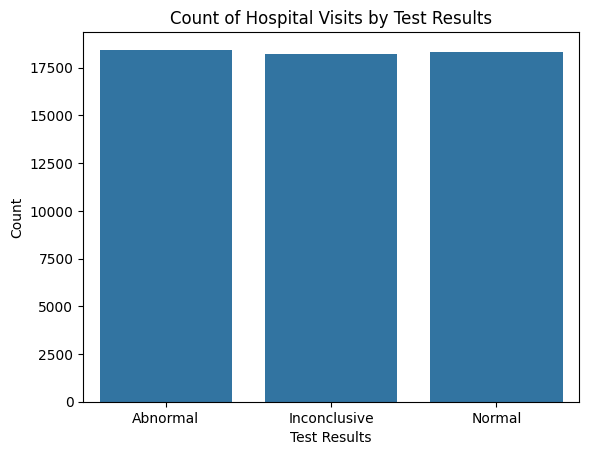
\includegraphics[width=0.5\textwidth]{image/test_results.png}
    \caption{Phân bố của kết quả dự đoán}
    \label{fig:test_result}
\end{figure}

\begin{figure}[h]
    \centering
    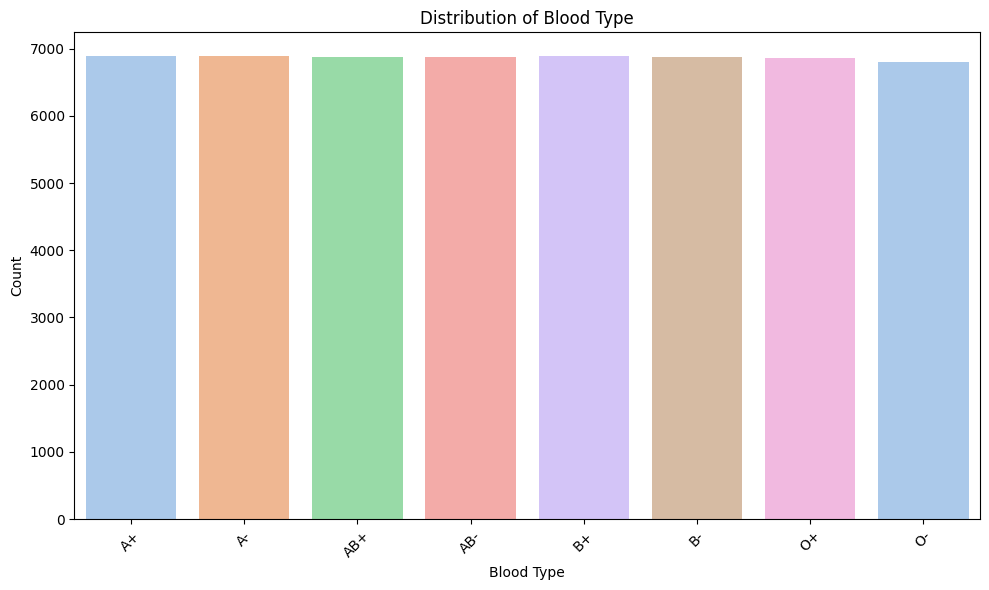
\includegraphics[width=0.5\textwidth]{image/blood.png}
    \caption{Nhóm máu}
    \label{fig:blood}
\end{figure}

\begin{figure}[h]
    \centering
    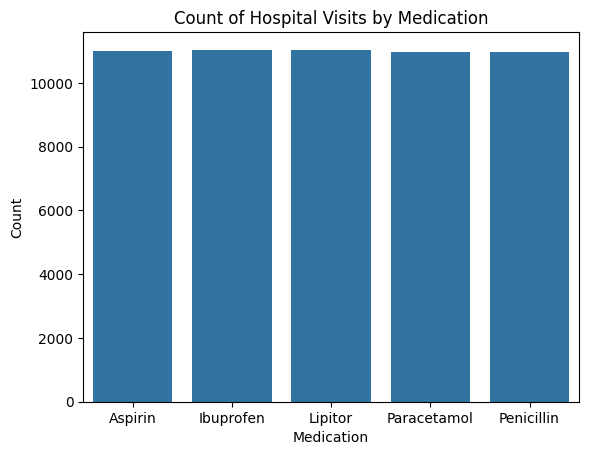
\includegraphics[width=0.5\textwidth]{image/medication.png}
    \caption{Các loại bảo hiểm}
    \label{fig:medication}
\end{figure}

\begin{figure}[hh]
    \centering
    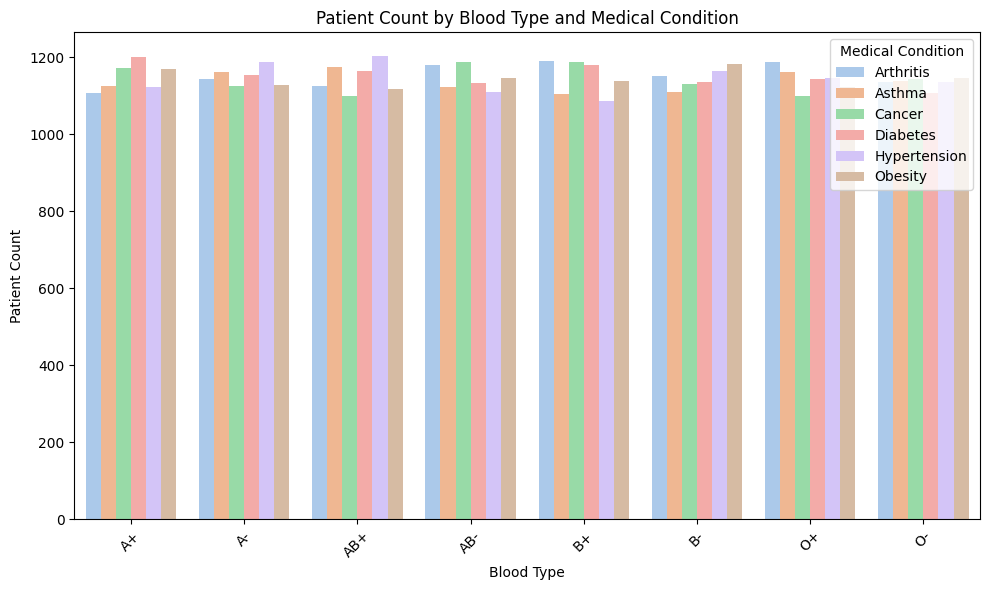
\includegraphics[width=0.5\textwidth]{image/mevsbl.png}
    \caption{Phân phối thuốc theo tình trạng bệnh lý}
    \label{fig:mevsbl}
\end{figure}


\section{Dự Đoán tình trạng sức khỏe}

\subsection{Sử Dụng Mô Hình Học Máy}
Để dự đoán kết quả sức khỏe người dùng, trong bài lab này sử dụng nhiều mô hình học máy khác nhau, bao gồm:
\begin{itemize}
    \item \textbf{Hồi quy tuyến tính (Linear Regression)}: Mô hình này được sử dụng để dự đoán kết quả sức khỏe người dùng dựa trên các biến số tuyến tính như năm và giá cả.
    \item \textbf{Hồi quy XGBoost (XGBoost Regression)}: Đây là một mô hình mạnh mẽ, có khả năng xử lý các dữ liệu phức tạp và tối ưu hóa quá trình dự đoán.
    \item \textbf{KNN cho hồi quy và phân loại (KNN Regression and Classification)}: Mô hình này dựa trên khoảng cách giữa các điểm dữ liệu để dự đoán kết quả sức khỏe người dùng.
\end{itemize}

\subsection{Phân Tích Hiệu Suất Mô Hình}
Chúng tôi đã đánh giá hiệu suất của các mô hình dự đoán thông qua các chỉ số như:

\begin{itemize}
    \item \textbf{Lỗi bình phương trung bình (Mean Squared Error - MSE)}: Đo lường mức độ sai lệch giữa giá trị dự đoán và giá trị thực tế.
    \item \textbf{Độ chính xác (Accuracy Score)}: Đặc biệt quan trọng đối với mô hình phân loại, đánh giá khả năng dự đoán chính xác xu hướng tiêu dùng.
\end{itemize}

\begin{figure}[h]
    \centering
    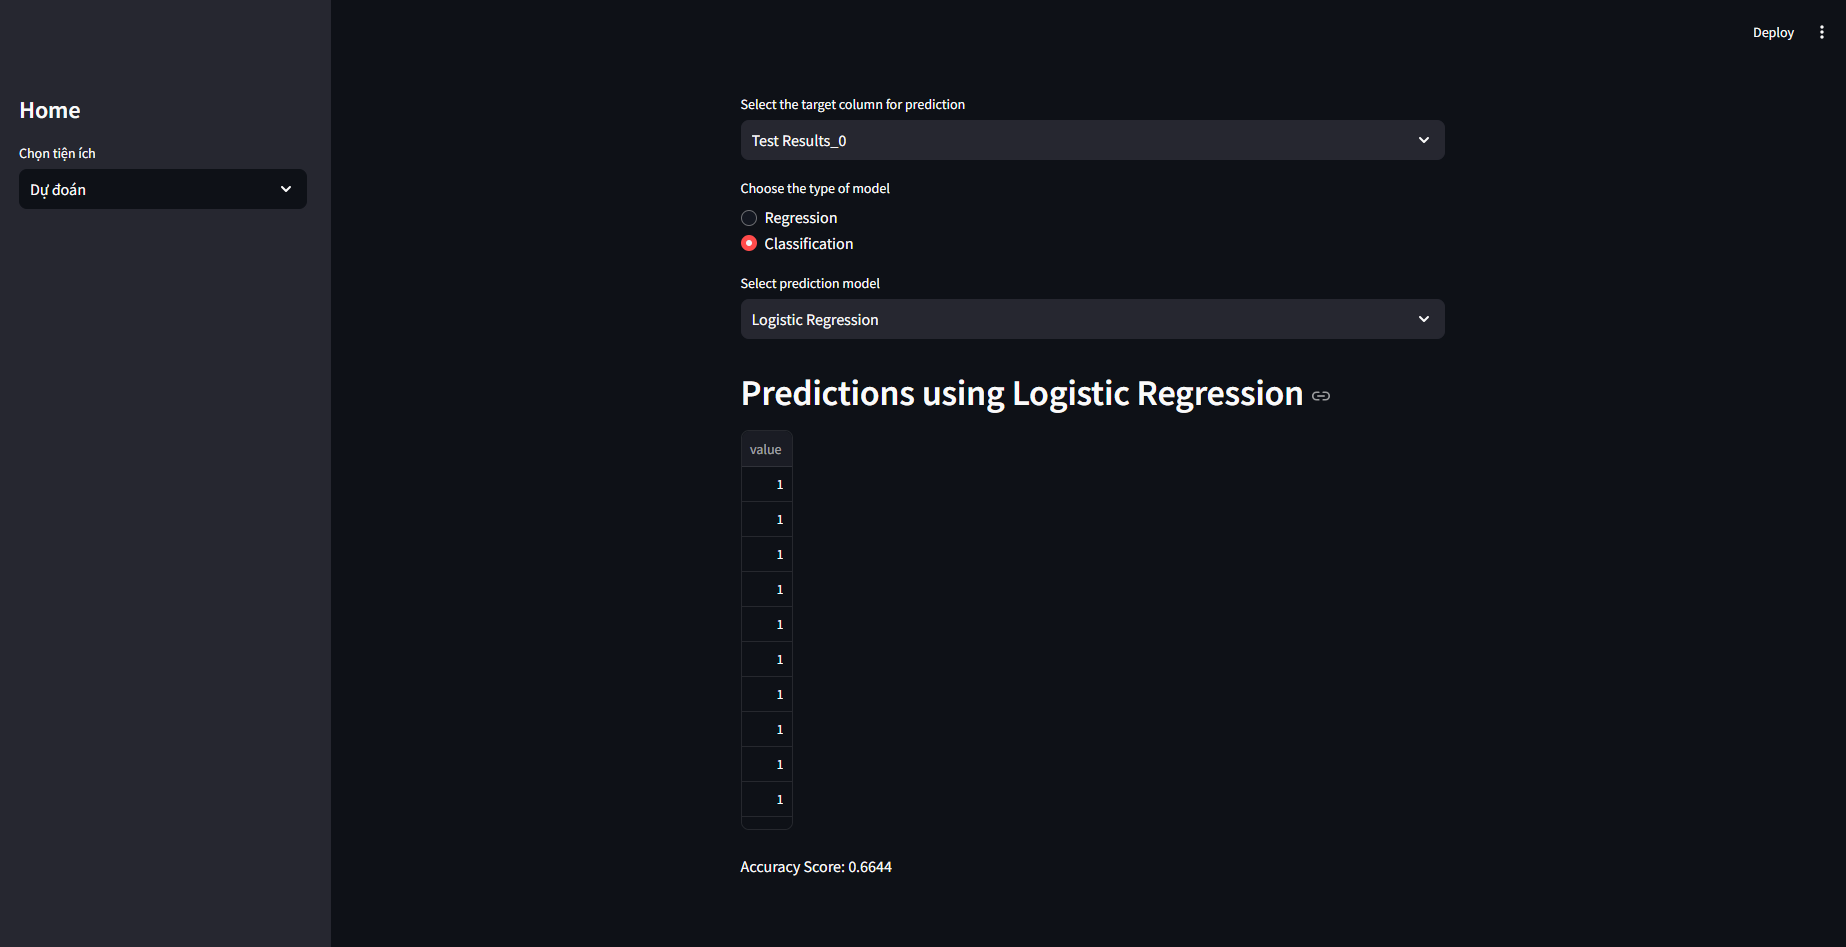
\includegraphics[width=0.5\textwidth]{image/predict_logi.png}
    \caption{Dự đoán kết quả với Logistic, cho được kết quả 0.6644 }
    \label{fig:predict}
\end{figure}

Kết quả cho thấy mô hình XGBoost mang lại độ chính xác cao hơn so với các mô hình khác, đặc biệt khi dữ liệu có tính phức tạp và biến động lớn.

\section{Tích Hợp Chatbot Hỗ Trợ Dự Đoán}

\subsection{Tích Hợp Chatbot}
Để hỗ trợ người dùng trong việc truy vấn xu hướng tiêu dùng, chúng tôi đã tích hợp chatbot vào hệ thống. Chatbot này không chỉ trả lời các câu hỏi về xu hướng hiện tại mà còn sử dụng các mô hình học máy để dự đoán xu hướng tương lai. Chatbot giúp người dùng dễ dàng truy vấn dữ liệu và tìm hiểu về các xu hướng tiêu dùng trong ngành công nghệ.

\subsection{Mã Python tích hợp chatbot}
Dưới đây là một ví dụ về mã Python tích hợp chatbot:

\begin{verbatim}
import streamlit as st
import google.generativeai as genai

def chatbot_response(chat, message, history):
    system_message = "Bạn là chuyên gia về xu hướng tiêu dùng sản phẩm công nghệ."
    context = "\n".join([f"{msg}: {resp}" for msg, resp in history])
    response = chat.send_message(system_message + "\n" + context + "Người dùng: " + message)
    return response
\end{verbatim}

Chatbot được tích hợp khả năng học từ các cuộc trò chuyện trước đó để cải thiện độ chính xác và tính cá nhân hóa trong quá trình phản hồi.

\section{Kết Luận}
Báo cáo này đã trình bày quá trình phân tích dữ liệu và dự đoán xu hướng tiêu dùng sản phẩm công nghệ thông qua các mô hình học máy. Việc tích hợp chatbot hỗ trợ dự đoán giúp người dùng dễ dàng truy vấn và tìm hiểu về các xu hướng tiêu dùng, đồng thời cung cấp các thông tin dự báo có giá trị cho các doanh nghiệp.


\chapter{Lab 4: Trực Quan Hóa Dữ Liệu Không Gian với Streamlit}

\section{Giới thiệu}
Trong Lab 4, chúng tôi đã phát triển một ứng dụng web sử dụng Streamlit để trực quan hóa dữ liệu không gian. Mục tiêu của lab này là xây dựng một hệ thống trực quan hóa mạnh mẽ, tích hợp phân tích dữ liệu lớn và trí tuệ nhân tạo (AI). Ứng dụng cho phép người dùng tương tác với các bản đồ địa lý và dự báo các xu hướng dựa trên mô hình học máy.

Ứng dụng này sử dụng các thư viện mạnh mẽ như Leafmap, Geemap, Pydeck, và Kepler.gl để tạo ra các bản đồ tương tác 3D, cung cấp cái nhìn trực quan và chi tiết về dữ liệu không gian. Đồng thời, chúng tôi tích hợp các mô hình Machine Learning để dự đoán các yếu tố địa lý như mật độ dân số dựa trên dữ liệu.

\section{Phát triển Ứng dụng Streamlit}
\subsection{Tạo và quản lý giao diện Streamlit}
Ứng dụng được phát triển sử dụng Streamlit với giao diện đa trang cho phép người dùng dễ dàng tùy chỉnh dữ liệu và hiển thị bản đồ. Streamlit cung cấp giao diện trực quan và dễ dàng cho việc tương tác với người dùng, giúp người dùng có thể xem, chọn và lọc dữ liệu một cách linh hoạt.

Dữ liệu được hiển thị theo thời gian thực và có khả năng cập nhật ngay lập tức khi người dùng thay đổi các tiêu chí lọc.

\section{Xây dựng bản đồ tương tác}
\subsection{Tạo bản đồ 3D với Pydeck}
Ứng dụng của chúng tôi sử dụng Pydeck và Kepler.gl để xây dựng các bản đồ tương tác 3D. Các bản đồ này cho phép người dùng khám phá các dữ liệu địa lý không gian một cách trực quan và sinh động. Các dữ liệu từ OpenStreetMap và Kaggle được tích hợp để tạo ra các bản đồ đa chiều, có thể tương tác theo thời gian thực.

\begin{figure}[h]
    \centering
    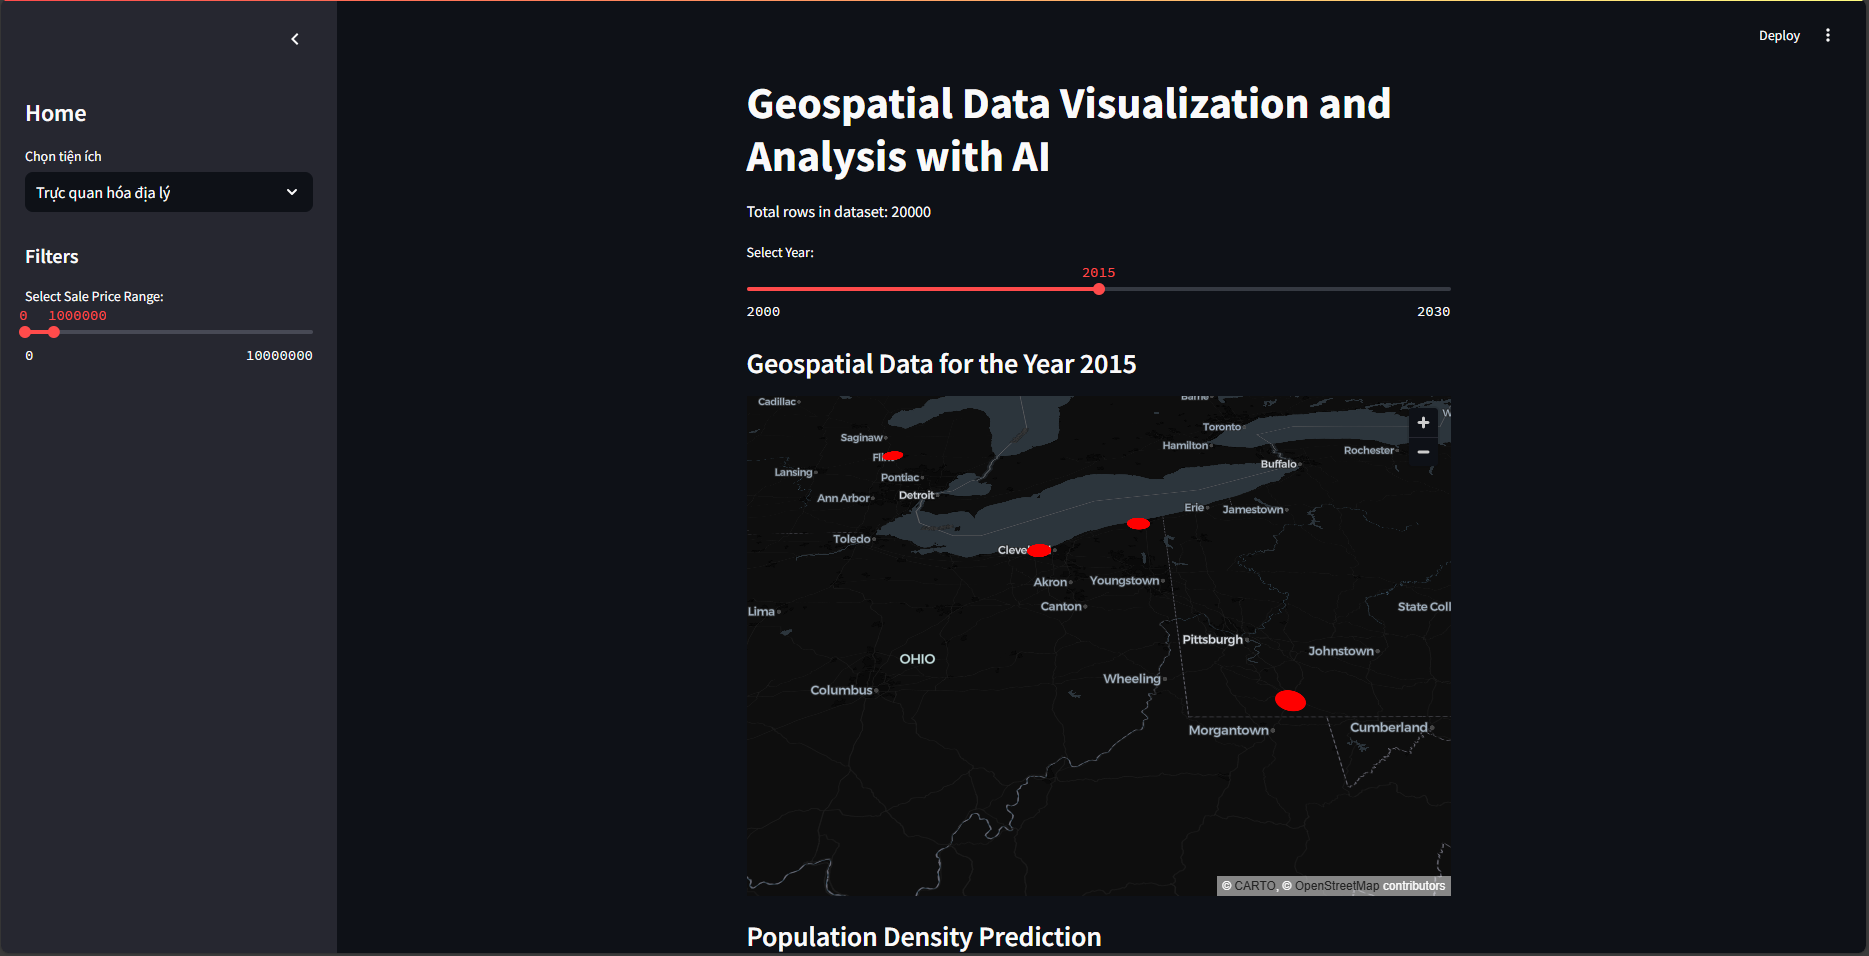
\includegraphics[width=0.5\textwidth]{image/geo_ui.png}
    \caption{Giaop diện của bản đồ}
    \label{fig:geo}
\end{figure}

Mỗi khi người dùng thay đổi các bộ lọc hoặc lựa chọn một khu vực khác trên bản đồ, các bản đồ sẽ tự động cập nhật để hiển thị dữ liệu mới nhất. Điều này cho phép người dùng dễ dàng phân tích các xu hướng không gian, chẳng hạn như mật độ dân số hoặc giá bất động sản theo từng khu vực.

\section{Phân tích Dữ liệu Lớn và Mô Hình Hóa AI}
\subsection{Xử lý dữ liệu lớn với Dask}
Trong lab này, chúng tôi xử lý các bộ dữ liệu lớn với hơn 1 triệu dòng bằng cách sử dụng Dask. Dask cho phép chúng tôi phân tích dữ liệu mà không cần tải toàn bộ vào bộ nhớ, giúp ứng dụng có thể xử lý hiệu quả hơn với các bộ dữ liệu lớn.

\subsection{Dự báo với Machine Learning}
Một tính năng quan trọng của ứng dụng là khả năng dự báo mật độ dân số và các yếu tố địa lý khác dựa trên mô hình học máy. Chúng tôi đã sử dụng mô hình \textit{Random Forest Regressor} để dự đoán mật độ dân số dựa trên các biến số như kinh độ, vĩ độ và năm.

Dưới đây là một đoạn mã minh họa cách dự đoán mật độ dân số:

\begin{verbatim}
from sklearn.model_selection import train_test_split
from sklearn.ensemble import RandomForestRegressor

# Xây dựng mô hình dự đoán mật độ dân số
def predict_population_density(X):
    data = pd.DataFrame({
        'lon': np.random.rand(100) * 100,
        'lat': np.random.rand(100) * 100,
        'year': np.random.randint(2000, 2021, size=100),
        'population_density': np.random.rand(100) * 1000
    })
    
    X_train, X_test, y_train, y_test = train_test_split(data[['lon', 'lat', 'year']], data['population_density'], test_size=0.2, random_state=42)
    
    # Xây dựng mô hình
    model = RandomForestRegressor()
    model.fit(X_train, y_train)
    
    # Dự đoán
    prediction = model.predict(X)
    return prediction
\end{verbatim}

Mô hình này cho phép người dùng nhập vào các tọa độ địa lý và năm để dự đoán mật độ dân số cho khu vực đó.

\section{Hiển thị dữ liệu và kết quả dự đoán}
\subsection{Hiển thị dữ liệu tương tác theo thời gian thực}
Người dùng có thể tương tác với dữ liệu và bản đồ bằng cách sử dụng các thanh trượt và bộ lọc để chọn khoảng thời gian hoặc giá trị mong muốn. Kết quả sẽ được cập nhật ngay lập tức trên giao diện người dùng, giúp họ có cái nhìn trực quan về các xu hướng không gian.

\subsection{Kết quả dự đoán mật độ dân số}
Sau khi người dùng nhập vào các thông tin như kinh độ, vĩ độ và năm, ứng dụng sẽ sử dụng mô hình học máy để dự đoán mật độ dân số cho khu vực đó. Kết quả dự đoán sẽ được hiển thị ngay lập tức trên giao diện.

\begin{figure}[h]
    \centering
    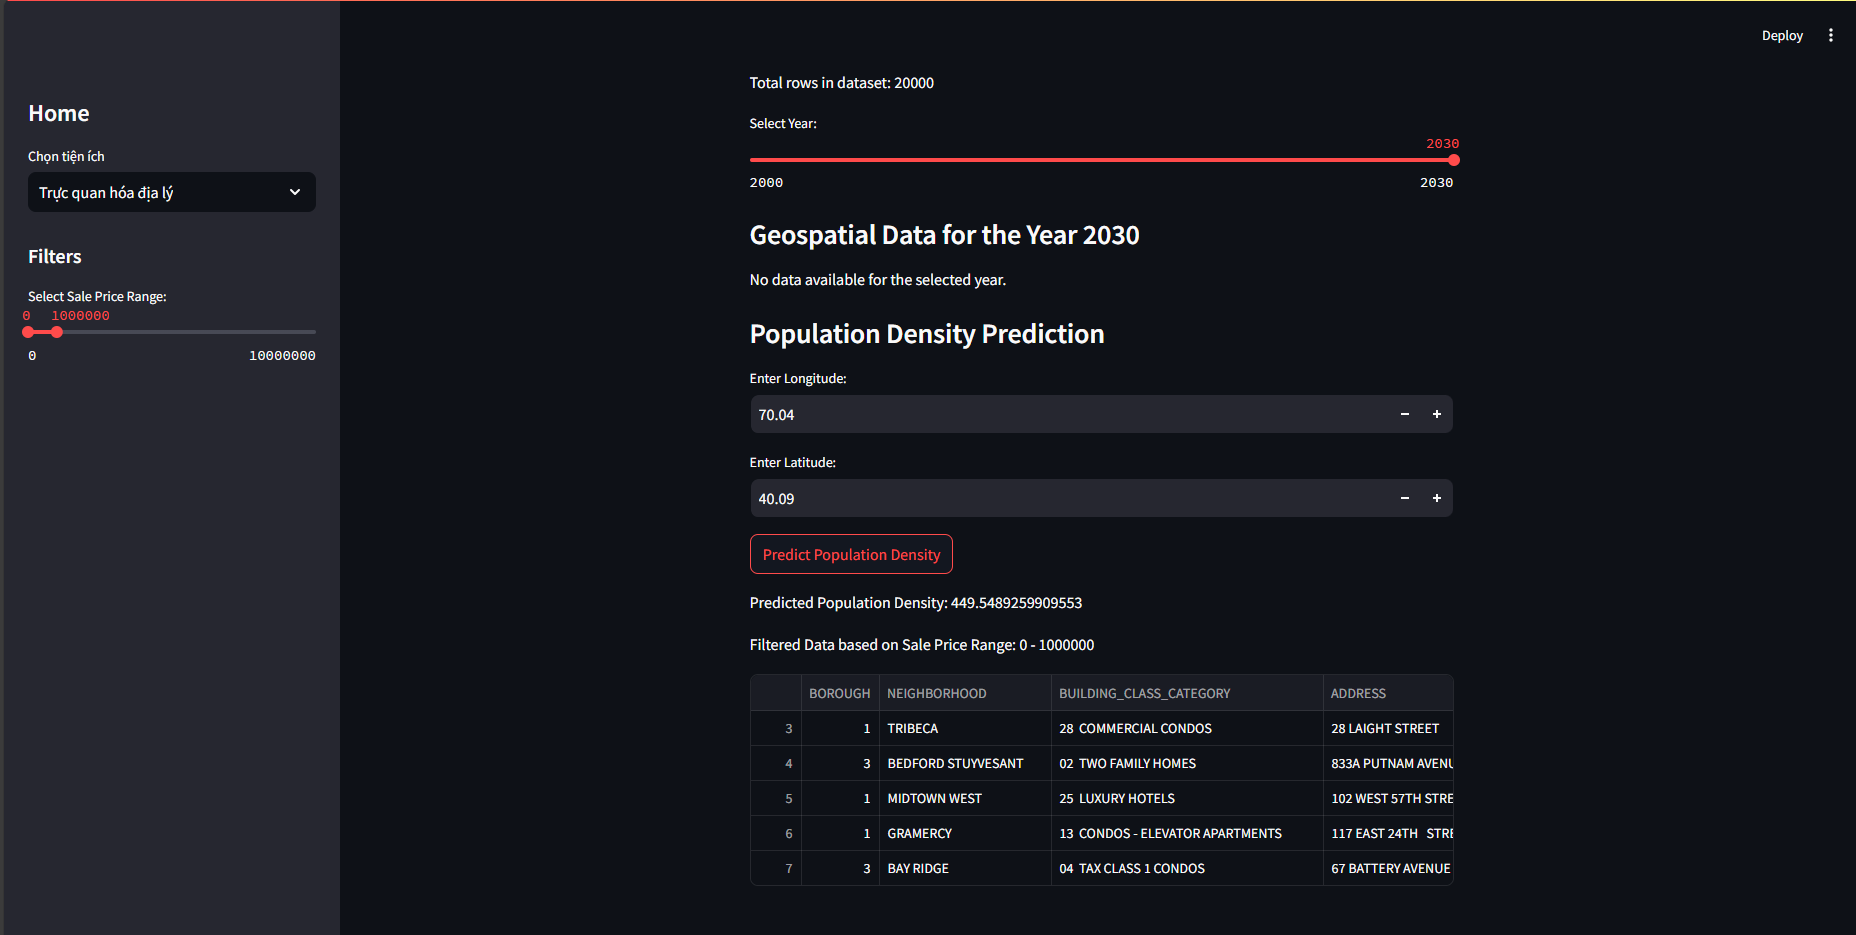
\includegraphics[width=0.5\textwidth]{image/predict_population.png}
    \caption{Mô hình dự đoán mật độ dân số các năm trong tương lai}
    \label{fig:population}
\end{figure}

\chapter{Kết Luận}
Trong suốt quá trình thực hiện các Lab từ 1 đến 5, chúng tôi đã tích lũy được nhiều kiến thức và kỹ năng quan trọng trong lĩnh vực phát triển hệ thống chatbot, phân tích và dự báo xu hướng, cùng với trực quan hóa dữ liệu không gian. Mỗi Lab đều đóng vai trò quan trọng trong việc xây dựng nền tảng và mở rộng các chức năng của hệ thống ứng dụng thông minh. Từ việc phát triển chatbot cơ bản trong Lab 1, đến mở rộng với các tính năng tư vấn sức khỏe trong Lab 2, chúng tôi đã học cách tích hợp cơ sở dữ liệu và cá nhân hóa trải nghiệm người dùng. Lab 3 cho phép chúng tôi áp dụng các mô hình học máy để phân tích xu hướng tiêu dùng sản phẩm công nghệ, trong khi Lab 4 giúp chúng tôi phát triển ứng dụng Streamlit mạnh mẽ cho trực quan hóa dữ liệu không gian. Cuối cùng, Lab 5 là sự tổng hợp của tất cả các kỹ năng đã học, tạo ra một ứng dụng hoàn chỉnh và đa chức năng, kết hợp giữa tư vấn thông minh, dự báo dựa trên AI và trực quan hóa dữ liệu hiệu quả. Từ đó, chúng tôi nhận ra giá trị của việc kết hợp công nghệ và dữ liệu để giải quyết các vấn đề thực tiễn trong nhiều lĩnh vực.

\end{document}
